% See exam.cls and examdoc.tex for the license information
\documentclass[12pt, answers]{exam}

\usepackage{amssymb}
\usepackage{makeidx}
\usepackage{amsmath}
\usepackage{graphicx}
\usepackage{caption}
\usepackage{tabulary}
\usepackage{color}
\usepackage{multicol}
%\usepackage{multirow}
%\usepackage{enumerate}

\usepackage{array}
\newcolumntype{C}[1]{>{\centering\let\newline\\\arraybackslash\hspace{0pt}}m{#1}}

\addpoints

% In case we're not using hyperref.sty:
\providecommand{\texorpdfstring}[2]{#1}
% The following can be used in \section commands
% without generating pdf warnings:
\newcommand{\bs}{\texorpdfstring{\char`\\}{}}

\makeindex

\newcommand{\indc}[1]{\index{#1@\texttt{\char`\\#1}}}
\newcommand{\indcsub}[2]{\index{#1@\texttt{\char`\\#1}!#2}}
\newcommand{\indcstart}[1]{\index{#1@\texttt{\char`\\#1}|(}}
\newcommand{\indcstop}[1]{\index{#1@\texttt{\char`\\#1}|)}}

\newcommand{\indt}[1]{\index{#1@\texttt{#1}}}
\newcommand{\indtsub}[2]{\index{#1@\texttt{#1}!#2}}
\newcommand{\indtstart}[1]{\index{#1@\texttt{#1}|(}}
\newcommand{\indtstop}[1]{\index{#1@\texttt{#1}|)}}

\extraheadheight{-.4in}

\pagestyle{headandfoot}
%\extraheadheight{.2 in}
\firstpageheader{}{}{}
\runningheader{}{}{}
\firstpagefooter{}{Extension of global alignment}{Page \thepage\ of \numpages}
\firstpagefootrule
\runningfooter{}{Extension of global alignment}{Page \thepage\ of \numpages}
\runningfootrule

%---------------------------------------------------------------------

\shadedsolutions
\noprintanswers
\definecolor{SolutionColor}{rgb}{0.8,0.9,1}

\setcounter{section}{2}

\begin{document}

\section{Exercises -- Extension of global alignment}

%---------------------------------------------------------------------
\begin{questions}

%%% Question 1
\question \textbf{DP with score matrix}
  
Use the score matrix below with gap penalty g =1 and answer the following questions.

\begin{figure}[h]
  \centering
      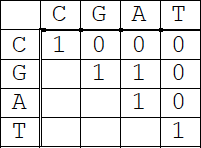
\includegraphics[width=0.2 \textwidth]{fig03/simple_score_matrix.png}
\end{figure}

\begin{parts}

%% (a)
  \part	Calculate the alignment score.

\begin{itemize}
\item Alignment 1
\begin{verbatim}
    q: ATGCT
    d: CA--T \end{verbatim}
    
\begin{solution}[0.35 in]
  1
\end{solution}
  
\item Alignment 2
\begin{verbatim}
    q: CAGCT
    d: C-A-T \end{verbatim}
  
\begin{solution}[0.35 in]
  1
\end{solution}

\end{itemize}

%% (b)
\part Use the simple scorning scheme and fill the empty cells with appropriate scores.

\begin{itemize}
\item Table A
\begin{figure}[h]
  \centering
      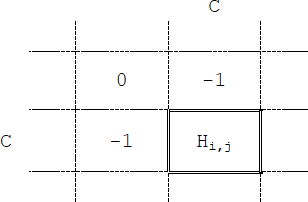
\includegraphics[width=0.25 \textwidth]{fig03/cell_update_score_matrix_1.png}
\end{figure}

\begin{solution}[0.75 in]
1
\end{solution}

\item Table B
\begin{figure}[!h]
  \centering
      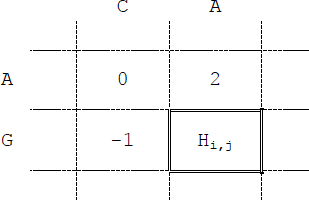
\includegraphics[width=0.25 \textwidth]{fig03/cell_update_score_matrix_2.png}
\end{figure}

\begin{solution}[0.75 in]
1
\end{solution}

\end{itemize}

\pagebreak

%% (c)
\part Fill the empty cells with appropriate scores in the DP table. What is the optimal alignment score?

\begin{figure}[h]
  \centering
      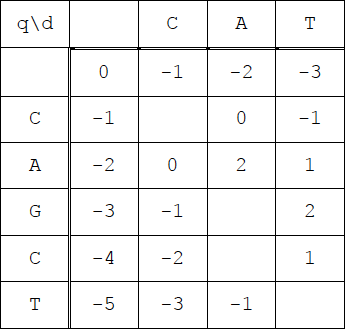
\includegraphics[width=0.35 \textwidth]{fig03/dp_with_score_matrix.png}
\end{figure}

\begin{solution}[0.75 in]
1
\end{solution}

%% (d)
\part There are two different alignments that give the same optimal score in the solution above. Specify both of them.

\begin{solution}[1.75 in]
\begin{verbatim}
  q: CAGCT
  d: CA--T
  
  q: CAGCT
  d: C-A-T
\end{verbatim}
\end{solution}

\end{parts}

\pagebreak


\end{questions}
%---------------------------------------------------------------------
       
\end{document}

